\begin{titlepage}
    \begin{tikzpicture}[remember picture,overlay]
    	% Franja
    	\fill[RoyalBlue]
    	($(current page.north)+(0,-2cm)$)
    	rectangle
    	($(current page.south)+(3pt,2cm)$);
 
    	% Logo
    	\node at ([xshift=2cm, yshift=-3cm]current page.north west)[anchor=west]{
\includegraphics[width=7cm, height=2cm, keepaspectratio]{img/LogoInsitel}};
	
    	% Reporte
    	\node at ($(current page.center)!0.5!(current page.north east)$){
        	\begin{tblr}{colspec={l}, hlines=0pt, vlines=0pt, column{1}={font=\large}, row{1}={bg=white, font=\LARGE\bfseries, fg=RoyalBlue}}
            	\SetCell{8cm} REPORTE DE MANTENIMIENTO:\\
            	\SetCell{8cm} REPORTE DE MANTENIMIENTO REALIZADO A LA ESTACIÓN ACELEROMÉTRICA INSTALADA EN EL EDIFICIO \textit{\Large\color{RoyalBlue}``\MakeUppercase{\edificio}''}
        	\end{tblr}
 
    	};
	
    	% Datos
    	\node[yshift=5cm] at ($(current page.center)!0.5!(current page.south west)$){
        	\begin{tblr}{colspec={r}, hlines=0pt, vlines=0pt, row{1,5,8,11}={bg=white, fg=RoyalBlue, font=\large\bfseries}}
            	ELABORADO POR:\\
            	Oficina Técnica INSITEL\\
            	N° de folios: \pageref{LastPage}\\
            	\\
            	CONTRATISTA:\\
            	Instrumentación Sísmica y Telemetría SAC - INSITEL\\
            	\\
            	CLIENTE:\\
            	\\
            	\\
            	REPORTE DE MANTENIMIENTO:\\
            	N° RPMNTTO-2026-0\nroinforme
        	\end{tblr}
    	};
	
    	% Firma
    	\node at ($(current page.center)!0.5!(current page.south east)$){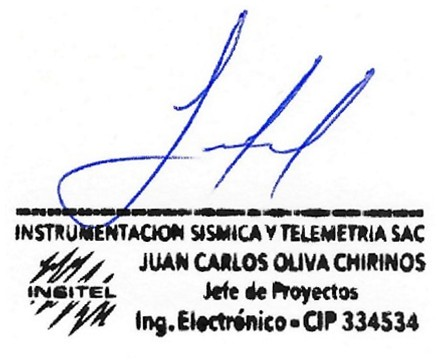
\includegraphics[width=3.6cm, height=3cm, keepaspectratio]{img/FirmaJuanCarlos}};
	
    	% Pie
    	\node[yshift=1cm, font=\bfseries] at (current page.south){INSITEL | Lima - Perú - 2026};
    \end{tikzpicture}
\end{titlepage}
